\chapter{OLAP and Graph Databases}
% ---
This chapter introduces the main concepts that forms the theoretical foundation necessary to better understand the work presented in this dissertation. Initially, we will explore the definition of Data Warehouse, Multidimensional Model and OLAP tools. Then, we will dive into concepts related to Graph and Graph Databases.

\section{Data Warehouse}
According to \cite{Inmon2005}, a data warehouse (DW) is ``a subject-oriented, integrated, nonvolatile, and time-variant collection of data in support of management's decisions''. The first important aspect of a data warehouse is that it is subject-oriented, which means that the information stored in the DW is related to the company's subject. Consider a retail company for example: the main subjects can be product, sale, vendor and customer, therefore the data in the warehouse will be related to these entities.
 
The second characteristic of a data warehouse is that it is integrated, which means it contains data coming from multiple different sources. During the process of loading the warehouse, the data is converted, formatted, normalised and go through any other process to make the final information stored in the warehouse consistent. Another important aspect of a data warehouse is that it is nonvolatile, which means that the data in the warehouse does not get updated as operational environment. The warehouse is loaded in batches and it stores a snapshot, creating a history of the data. The final important aspect of a DW is that every record of data contains some sort of a time attribute to mark the moment in which the record is accurate.
 
Figure \ref{fig:figure1} shows the basic elements of a data warehouse \cite{Kimball2011}. The Operational Source Systems capture and store the transactions of the business and they are considered elements outside of the data warehouse, since there is no control on the content or the format of the data that they store. The Data Staging Area is where the process of Extract-Transformation-Load (ETL) is made: the data is extracted from the operational source system, then they are transformed in order to integrate all the information in a consistent format, and finally the data is loaded into the presentation area.

\begin{figure}[ht]
\centering
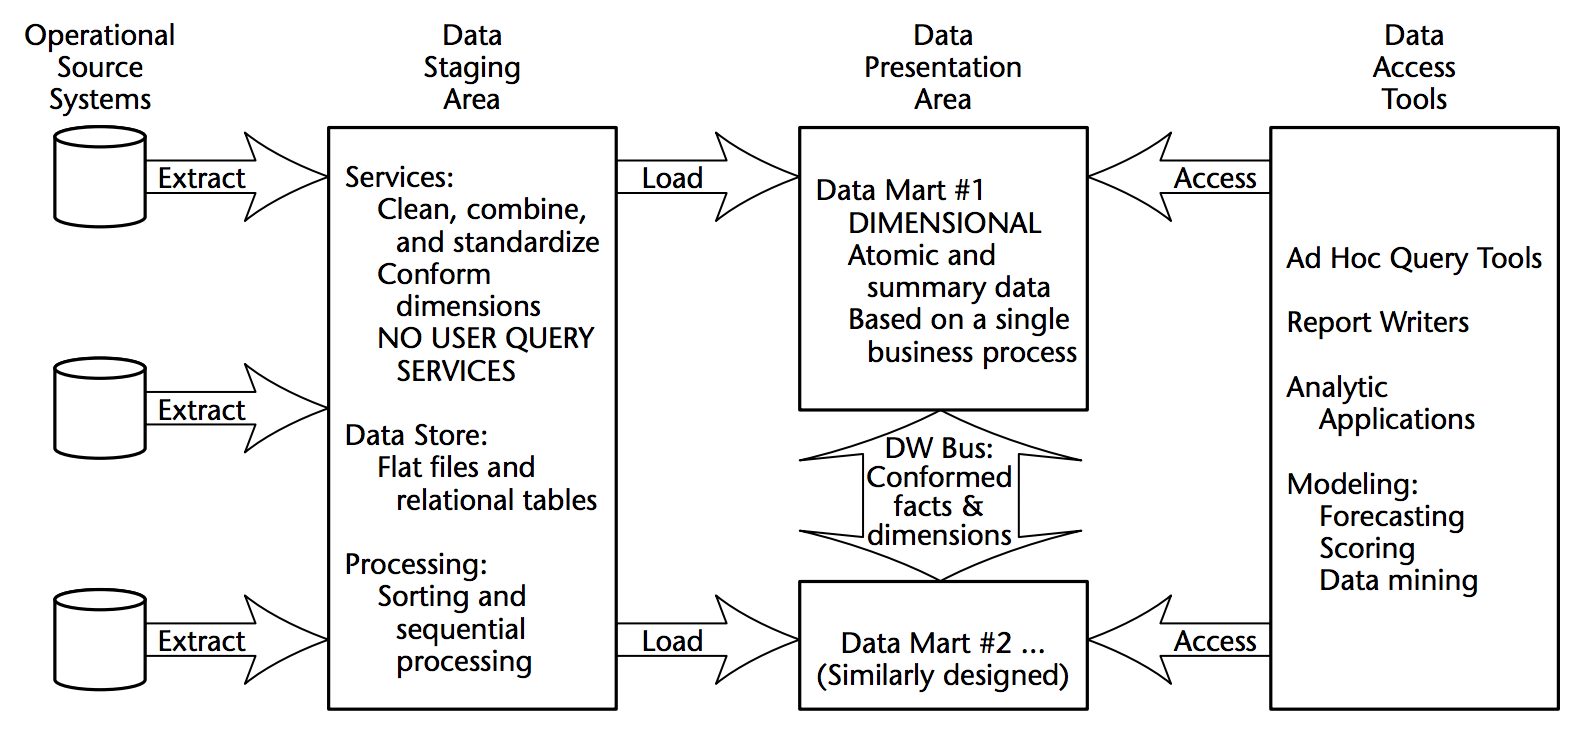
\includegraphics[width=.8\textwidth]{../elements_data_warehouse.png}
\caption{Elements of a Data Warehouse \cite{Kimball2011}}
\label{fig:figure1}
\end{figure}
 
The Data Presentation Area is where the data is organised, stored and accessed by analytical applications. According to \cite{Kimball2011}, this area should be composed by a series of integrated data marts, which are repositories that present the data for a single process of the organisational business. A data mart stores atomic data and organizes them in a model that is more legible to humans. The most popular technology used to implement data marts adopted by the industry is On-Line Analytical Processing (OLAP), that will be covered in more detail along this chapter. 

Finally, the Data Access Tools query the data in the presentation area. This element is formed by a set of different applications, from simple ad hoc queries until complex data mining application.

\section{Multidimensional Model}
The main functionality of a data warehouse is to facilitate multidimensional analysis \cite{OLAPCouncil}. This type of analysis reduces the number of misinterpretations by aligning the data with the analyst's mental model of the business. The multidimensional analysis provides an easy navigation through the database, showing specific subsets of data in different orientations and executing analytical calculations.
 
In order to perform multidimensional analysis, the data must be organised in a multidimensional model, where information is stored in a multidimensional array called \emph{hypercube} or \emph{cube} \cite{Vassiliadis1998}. A cube is composed by cells that store measures aggregated by the data dimensions. A \emph{dimension} is a cube's structural attribute formed by a list of properties that are similar to each other according to the user's perception of the data. Measures are the values being analysed by the user. Figure \ref{fig:figure2} shows an example of the dimensions and measures extracted from a sales application.

 
As shown in Figure \ref{fig:figure2} , each dimension (Geography, Time and Item) can be associated with an hierarchy of data aggregation levels. This feature allows user to view the data from different levels of details, for example: the measure \emph{Sales} aggregated by \emph{Region} can be detailed by \emph{Country} or even further detailed by \emph{City}.

\begin{figure}[ht]
\centering
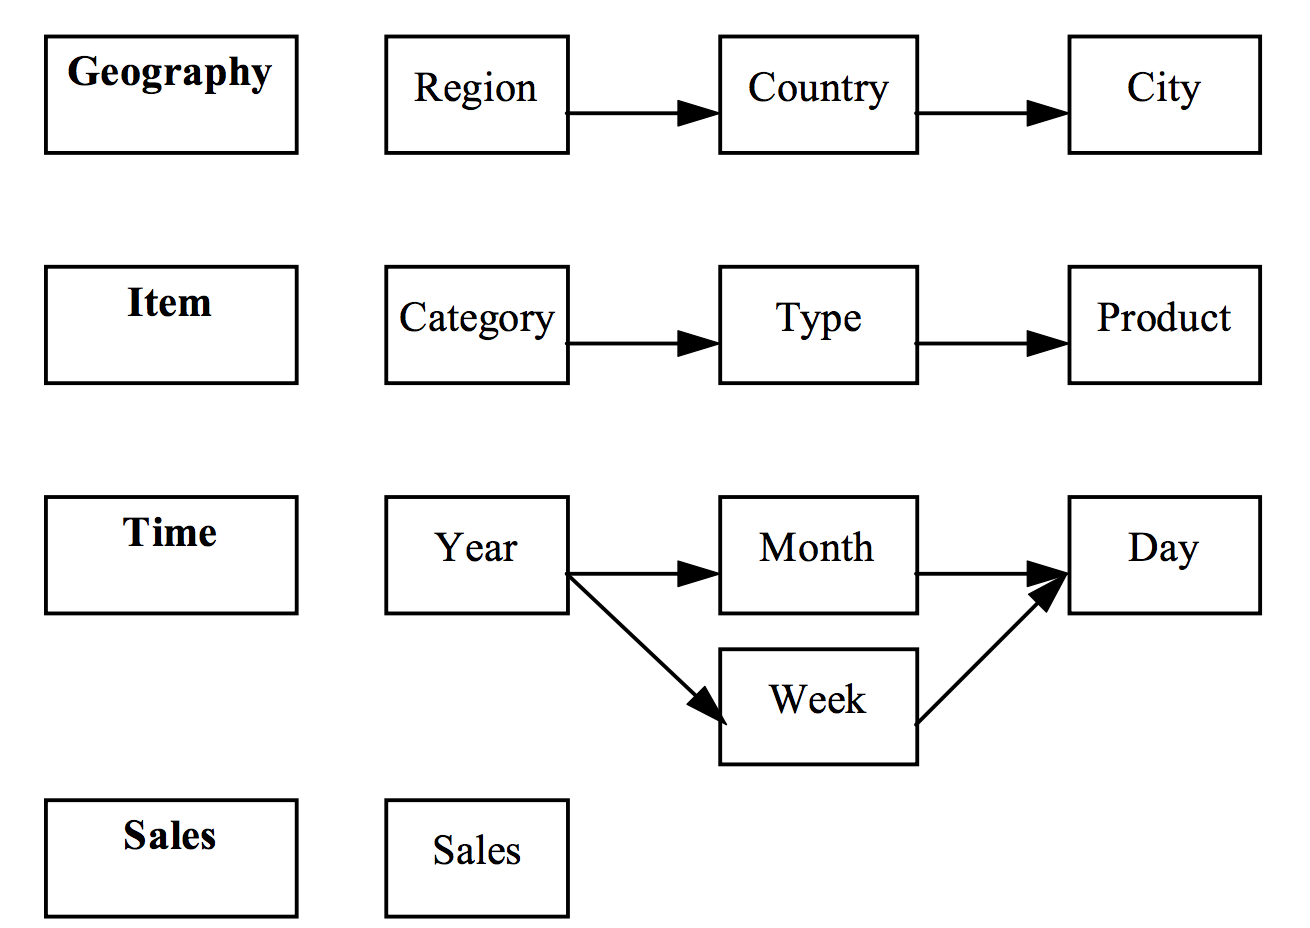
\includegraphics[width=.6\textwidth]{../dimensions_measures_example.png}
\caption{Example of dimensions and measure for a sales application  \cite{Vassiliadis1998}}
\label{fig:figure2}
\end{figure}

\section{OLAP}
On-Line Analytical Processing (OLAP) is a category of technological tools used by analysts and managers to extract new knowledge from consolidated enterprise data \cite{OLAPCouncil}. In order to achieve this goal, data are organised in cubes and stored following multidimensional models. The access to this data should be fast, consistent and interactive and it should provide various views of information, reflecting the different dimensions of an enterprise as perceived by the user.
 
Usually, the data loaded into an OLAP system comes from a data warehouse. According to \cite{Inmon2005}, the relationship between OLAP systems and data warehouse is complimentary: while OLAP offers control and flexible ways to explore data in different dimensions and hierarchy levels, data warehouse provides a robust data source for the OLAP system, where up-to-date data is available, already extracted and properly integrated.

\subsection{Types of OLAP Systems}
There are two approaches for the physical model of an OLAP system \cite{Vassiliadis1999}: Multidimensional On-Line Analytical Processing (MOLAP) and Relational On-Line Analytical Processing (ROLAP) Architectures.The MOLAP architecture provides a direct multidimensional view of the data. This approach stores the data in a Multidimensional Database Management System (MDBMS), which uses n-dimensional arrays that contains the measures of the cube. This type of DBMS has a better performance than traditional Relational Databases, but it is more difficult to manage updates.
 
The ROLAP architecture is a multidimensional interface to relational data. This approach uses a traditional Relational Database Management System (RDBMS) to store the data organised in a star or snowflake schema. A star schema is formed by one or more dimension tables and one centralised fact table, which stores the measures of interest for the OLAP system. Figure \ref{fig:figure3} shows an example of a star schema, where the tables TIME, GEOGRAPHY, ACCOUNT and PRODUCT are dimension tables and SALES is the fact table.

\begin{figure}[ht]
\centering
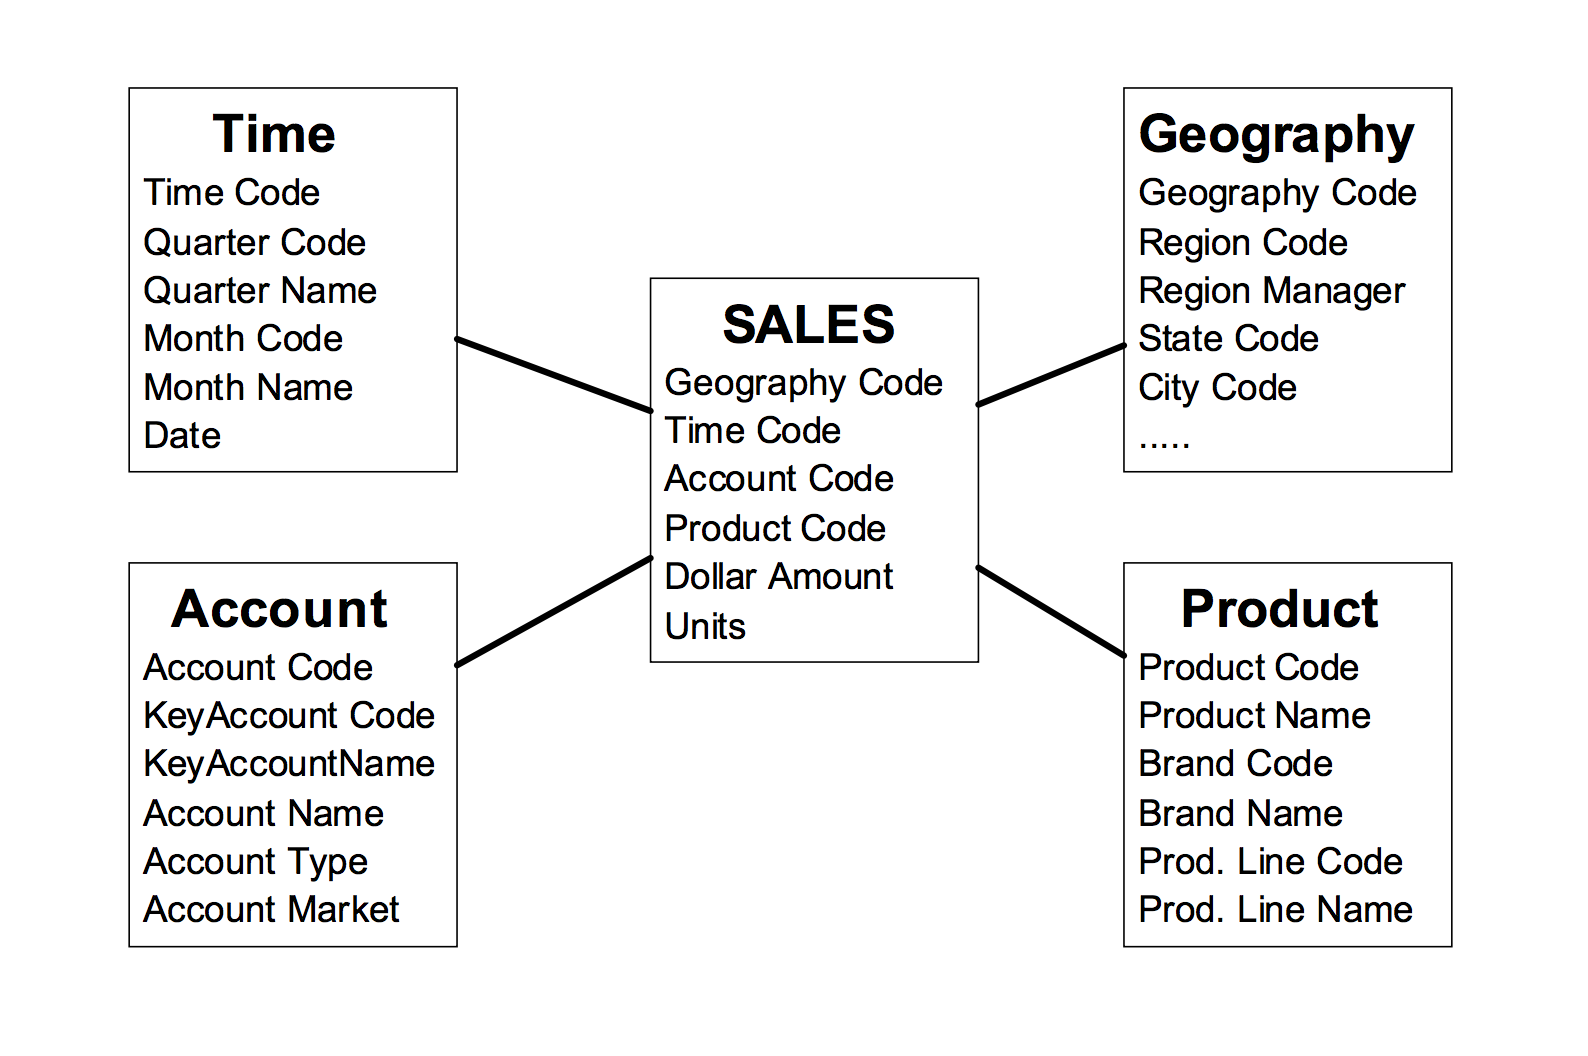
\includegraphics[width=.8\textwidth]{../star_schema_example.png}
\caption{Example of a Star Schema  \cite{Vassiliadis1999}}
\label{fig:figure3}
\end{figure}

Despite MOLAP architecture has the advantage of relying on a multidimensional native storage mechanism, the ROLAP approach allows easy integration with existing relational database systems and has the advantage of relational data being more efficiently stored than multidimensional data.

\subsection{OLAP Operators}
As mentioned earlier in this chapter, an OLAP system should provide a fast and interactive way for the user to explore the data stored in the cube. These are the main OLAP operations that can be used to navigate and manipulate different dimensions of the data \cite{Vassiliadis1998}:

\begin{description}
\item[Roll-up] Aggregates information along one dimension, summarising data on a higher level in its hierarchy. Consider the dimensions shown in Figure \ref{fig:figure2} and the measure of total dollar amount of sales per city, we can perform a roll-up operation to obtain the total dollar amount of sale per state.
\item[Drill-down] Detail information along one dimension, navigating the data from a higher to a lower hierarchy. Consider the measure of total dollar amount of sales per year, we can drill-down this query to obtain the total dollar amount of sales per month.
\item[Slice] Selects a slice of the cube according to user-specified dimension values. For instance, the user can select to view the total dollar amount of sales for the year of 2016.
\item[Dice] Selects a subcube from the original data according to user-specified conditions referred to more than one dimension. For instance, the user can select to view the total dollar amount of sales for the year of 2016 in the city of Recife.
\item[Pivot] Changes the orientation of dimensions in the cube, i.e. swap a row dimension to a column dimension.
\end{description}

There are other operations that can be performed in a OLAP system, but the ones shown above are considered the basic set of operations to support dynamic multidimensional analysis \cite{Inmon2005}.

\section{Graph}
Graph is a data structure formed by a set of vertices $V = \{v_1, \dots, v_n\}$  and a set of pair of vertices called edges $E = \{v_1v_2, \dots, v_nv_m\}$. It can be represented graphically (where the vertices are shown as circles and edges are shown as lines, as shown in Figure \ref{fig:figure4}) or mathematically in the form $G = (V, E)$ \cite{Tobergte2013}.

\begin{figure}[ht]
\centering
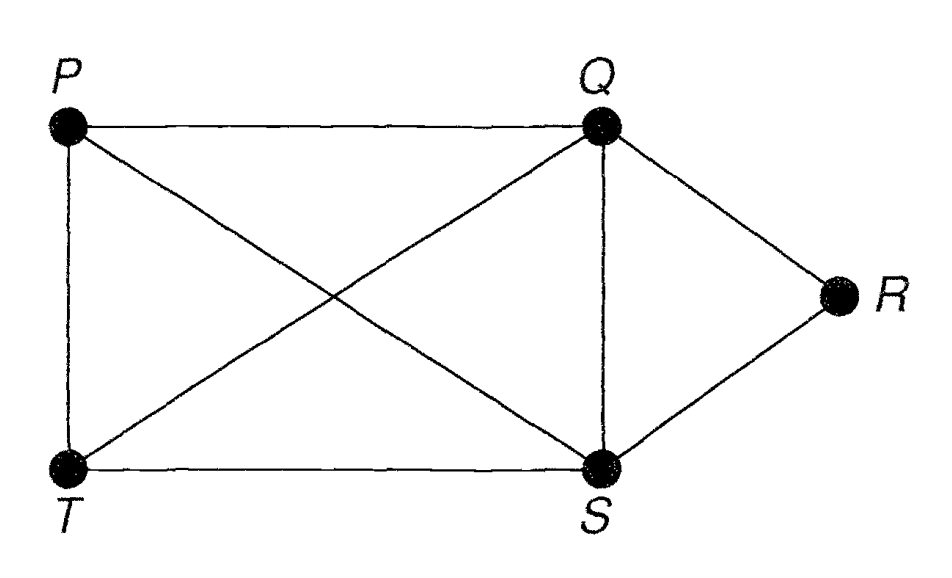
\includegraphics[width=.4\textwidth]{../graph_example.png}
\caption{Example of graph \cite{Tobergte2013}}
\label{fig:figure4}
\end{figure}

There are several real world applications that can take advantage of a graph model, specially the ones where the relationship between entities is an important information to be represented \cite{Miller2013}. Consider, for example, a social network application similar to Twitter, where a user can follow another user. In this scenario, we can represent a user as a vertex and the relationship between users as an edge, as shown in Figure \ref{fig:figure5}

\begin{figure}[ht]
\centering
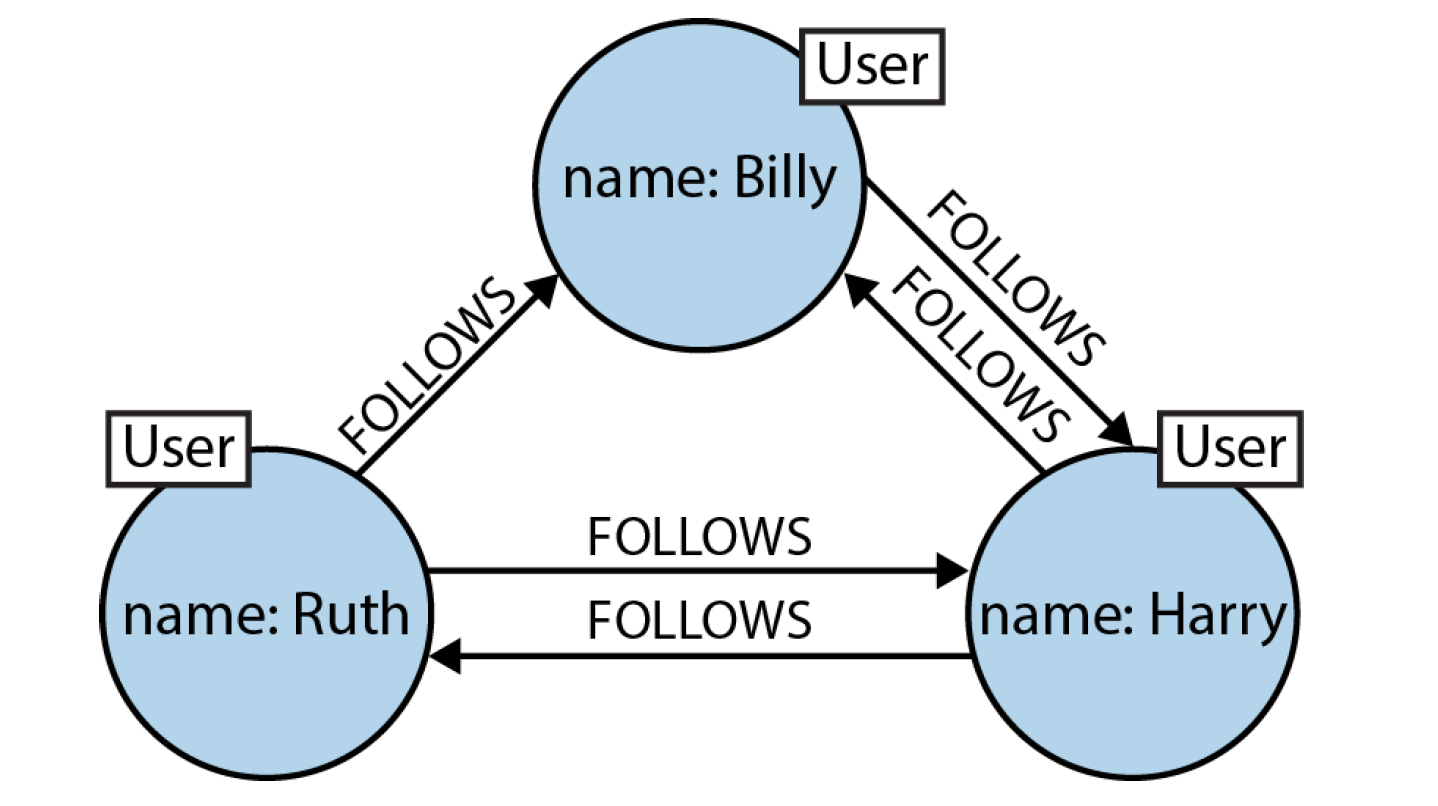
\includegraphics[width=.5\textwidth]{../social_network_graph_example.png}
\caption{Example of graph representation of a social network \cite{Miller2013}}
\label{fig:figure5}
\end{figure}

\subsection{Graph Theory}
Graph Theory is a branch of Mathematics dedicated to the study of graph structures \cite{Tobergte2013}. Given the definition of a general graph explained above, there are several classifications and concepts associated with graph structures.

\begin{description}
\item[Loop] When an edge starts and finishes in the same vertex, as the one shown in Figure \ref{fig:figure6} starting at vertex $T$ and finishing at vertex $T$.
\item[Multigraph] When a graph allows multiple edges connecting the same pair of vertices, as illustrated in Figure \ref{fig:figure6} with two edges connecting vertices $Q$ and $R$.

\begin{figure}[ht]
\centering
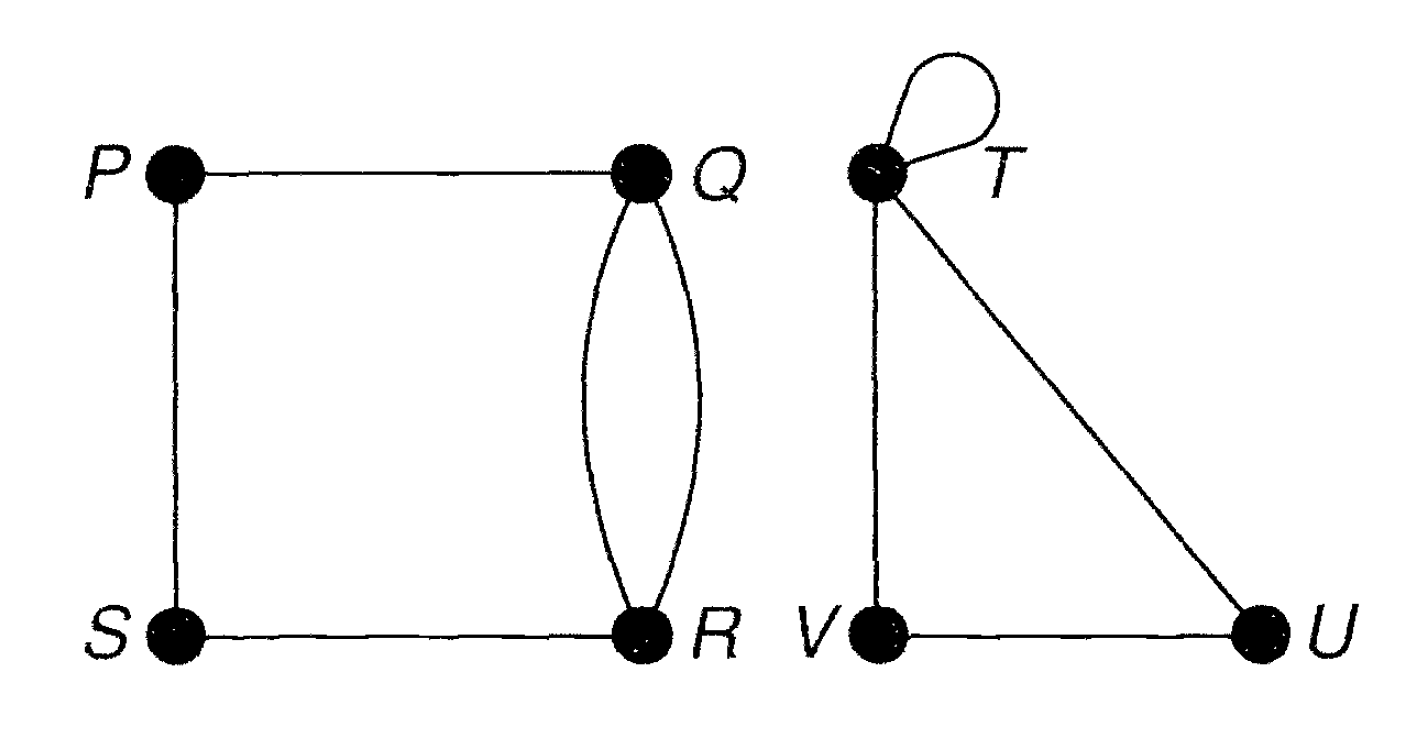
\includegraphics[width=.4\textwidth]{../loop_multigraph_example.png}
\caption{Example of a multigraph with a loop \cite{Tobergte2013}}
\label{fig:figure6}
\end{figure}

\item[Simple Graph] When a graph does not have loops or multiple edges, as the one depicted in Figure \ref{fig:figure4}.
\item[Complete Graph] When each pair of distinct vertices are connected to each other, as shown in Figure \ref{fig:figure7}.

\begin{figure}[ht]
\centering
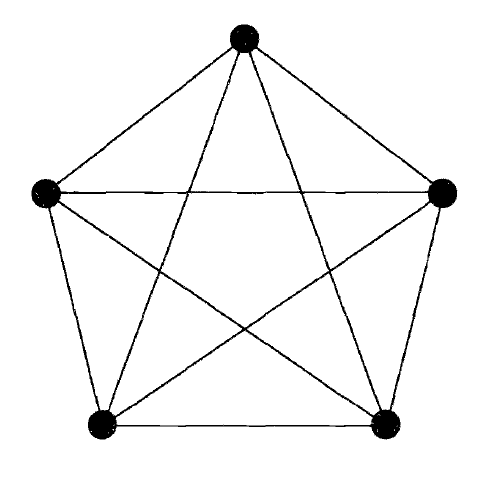
\includegraphics[width=.25\textwidth]{../complete_graph_example.png}
\caption{Example of a complete graph \cite{Tobergte2013}}
\label{fig:figure7}
\end{figure}

\item[Directed Graph] When the edges have directions expliciting the start and end of the connection, as illustrated in Figure \ref{fig:figure8}.

\begin{figure}[ht]
\centering
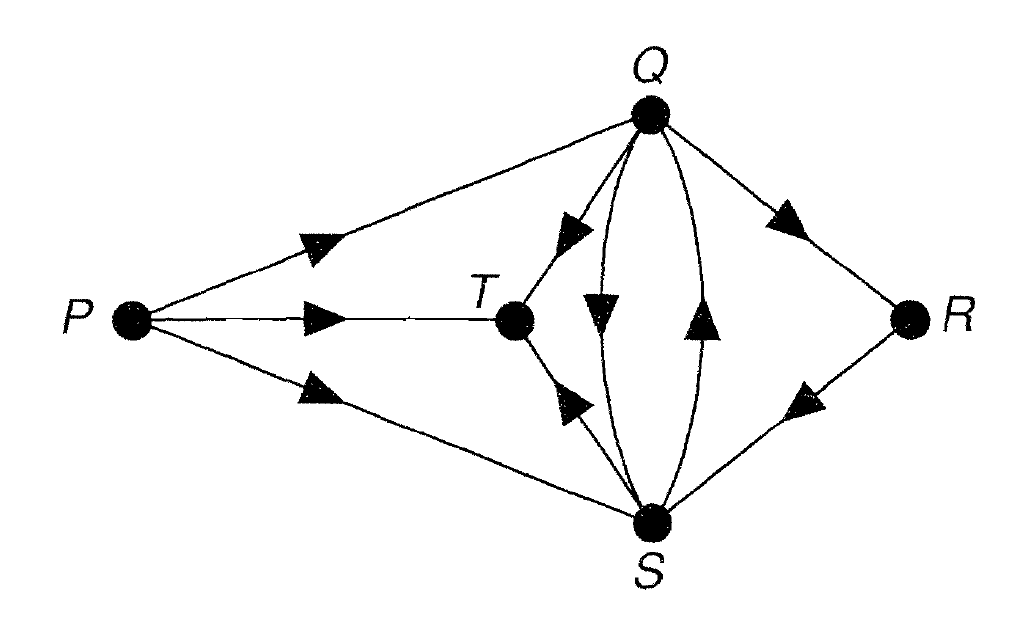
\includegraphics[width=.4\textwidth]{../directed_graph_example.png}
\caption{Example of a directed graph \cite{Tobergte2013}}
\label{fig:figure8}
\end{figure}

\item[Homogeneous Graph] It is a graph that has only one type of vertex.
\item[Heterogeneous Graph] It is a graph that has different types of vertices.
\item[Subgraph] It is a graph obtained from another graph $G$, where its vertices are a subset of the vertices of $G$ and its edges are a subset of the edges of $G$. Figure \ref{fig:figure9} shows in \ref{fig:figure9subfig2} a subgraph of the graph in \ref{fig:figure9subfig1}.
\item[Path] It is a subgraph obtained by a sequence of adjacent and distinct vertices.

\begin{figure}[ht]
\centering
\begin{subfigure}{.4\textwidth}
	\centering
	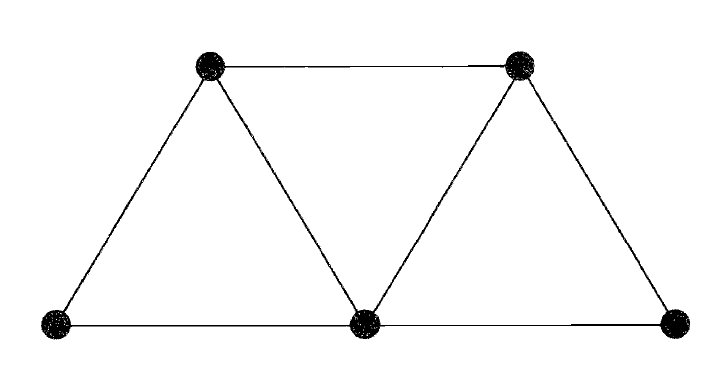
\includegraphics[width=.5\textwidth]{../subgraph_example_1.png}
	\caption{Original graph}
	\label{fig:figure9subfig1}
\end{subfigure} %
\begin{subfigure} {.4\textwidth}
	\centering
	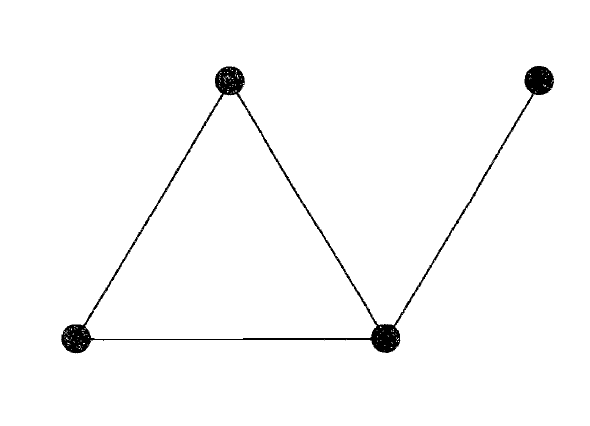
\includegraphics[width=.5\textwidth]{../subgraph_example_2.png}
	\caption{Subgraph}
	\label{fig:figure9subfig2}
\end{subfigure}
\caption{Example of a subgraph \cite{Tobergte2013}}
\label{fig:figure9}
\end{figure}
\end{description}
There are other types of classifications of a graph and other concepts associated to it \cite{Tobergte2013}. These are the main definitions for the purposes of understanding the work presented here.

\subsection{Network Analysis}

There are different kind of analysis that can be done depending on the nature of the graph data. Due to the work presented here, we will explore the aspects of social network analysis, which focus on the structure of relationships (edges) between entities (vertices) in the graph. Several types of analysis can be performed in a graph, but the measure of a vertex's centrality is historically one of the most studied cases of analysis \cite{Freeman1978}. A common application for a centrality measure is to find out what are the focal points in a social network, i.e. who are the people that are the most connected to other people? There are three types of centrality measures \cite{Freeman1978}:

\begin{description}
\item[Degree Centrality] This measure is given by the number of adjacent vertices. Formally, the Degree Centrality $C_D$ of a vertex $v_k$ can be given by

\begin{equation}
C_D(v_k) = \sum_{i=1}^{n} a(v_i, v_k),
\end{equation}

where $n$ is the total number of vertices in the graph and $a(v_i, v_k)$ is $1$ if and only if $v_i$ and $v_k$ are connected by one edge, or $0$ otherwise.

Considering a social network, a person (vertex) that has the greatest number of connections can be considered one of the focal points of the network, since it can directly read the most vertices in the graph. Given a graph with n vertices, the maximum value the degree centrality of a vertex in the graph can be is $n-1$. The degree centrality of a vertex is related to its potential communication activity.

\item[Betweenness Centrality] This measure is given by the frequency in which a vertex is present in the shortest path between other vertices. Formally, the Betweenness Centrality $C_B$ of a vertex $v_k$ is given by

\begin{equation}
C_B(v_k) = \sum_{i \neq j \neq k}^{n} \frac{\sigma_{ij}(v_k)}{\sigma_{ij}},
\end{equation}

where $\sigma_{ij}$ is the total number of shortest paths from vertex $v_i$ to vertex $v_j$ and $\sigma_{ij}(v_k)$ is the total number of shortest paths from $v_i$ to $v_j$ that passes through $v_k$.

Considering a social network, a person with high betweenness centrality is capable of influencing others by intercepting connections between several vertices in the graph. The betweenness centrality of a vertex is related to its potential control of communication.

\item[Closeness Centrality] This measure is given by the inverse of the sum distance of the shortest path of a vertex between other vertices in the graph. Formally, the Closeness Centrality $C_C$ of a vertex $v_k$ is given by

\begin{equation}
C_C(v_k) = \frac{1} {\sum_{i=1}^{n} d(v_i, v_k)}
\end{equation}

where $d(v_i, v_k)$ is the number of edges in the shortest path from $v_i$ to $v_k$.

Considering a social network, a person with high closeness centrality do not depend as much on others to communicate with other people in the network. The closeness centrality of a vertex is related to its potential independency and efficiency to control communication.
\end{description}

\section{Graph Databases}

Graph Databases are an alternative to Relational Database Management Systems (RDBMS), which are commonly used in the industry since the early 1980's. Despite the popularity of RDBMSs, GDBs allow the storage of data in graph model, which is a more natural way to represent information for some applications, such as social networks, semantic web pages and recommendation systems \cite{Miller2013}. 

The most popular form of graph model is the labeled property graph model \cite{Robinson2015}. The main characteristics of a labeled property graph are:
\begin{itemize}
\item Vertices and edges can contain properties, i.e. key-value pairs
\item Vertices can be labeled with one or more labels
\item Edges are labeled and directed, i.e. always have start and end vertices
\end{itemize}

The formal definition for a labeled property graph is given by $G = (V, E, L_V, L_E, A_V, A_E)$, where:
\begin{itemize}
\item $V$ is a set of vertices
\item $E \subseteq V \times V$ is a set of edges 
\item $L_V$ is a set of vertices labels and $L_E$ is a set of edge labels
\item $A_V = \{a_1, \dots, a_n\}$ is a set of vertex attributes, where $a_i = (k_i, m_i)$ is a key-value pair, $k_i$ is the attribute key and $m_i$ is the attribute value. Each vertex $v_i \in V$ is associated with a set of attributes. $A_E = \{b_1, \dots, b_n\}$ is the set of edge attributes defined in the same way as vertex attributes.
\end{itemize}

An example of a labeled property graph was shown in Figure \ref{fig:figure5}, where the vertices have the label ``User'' and the property ``name'' and the relationships are named ``Follows'' and have arrows indicating the direction of the edge.

\subsection{Historical Overview}

Scientific research related to graph data models were continuously published between 1980's and the first half of 1990's. Then, the database community attention turned to semistructured data model, due to the emergence of XML and the growth of hypertext document applications \cite{Angles2008}. From this period, the main focus of the graph databases proposed was to establish a better way to represent data and methods to retrieve and manipulate data modelled as graph.
 
Recently this area has gained again attention from the community, due to the emergence of trendy projects (chemistry, biology, social network, semantic web, among others) where the importance of information relies not only in the entities but also in the relationship between them \cite{Angles2012}. Most recent implementations of graph databases are concerned with handling increasing amount of data and improving performance in retrieving and manipulating data.
 
The most popular graph database system according to DBEngines\footnote{https://db-engines.com/en/system/Neo4j} website is Neo4J\footnote{https://neo4j.com/}. It is an open source native graph storage database system implemented in Java. Neo4J has its own query language called Cypher, which can be used to create, update and retrieve vertices and edges. This graph database system also provides high availability and scalability for big volume of graph data.

Besides Neo4J, there are other popular graph databases system according to DB Engine site. OrientDB\footnote{http://orientdb.com/orientdb/} is a NoSQL Multi-Model database, which means it stores data in the form of documents, key-value stores, objects, graph and others. Like Neo4J, OrientDB is also implemented in Java, but it uses an extended version of SQL that includes special operators to manipulate graph. This database system allows the creation of a pre-defined data schema and the definition of complex data type, like dates, decimals and binary objects (BLOB).
 
TitanDB\footnote{http://titan.thinkaurelius.com/} is a native graph database system implemented in Java. In order to establish connection with the hard disk, Titan needs to be linked to a data storage system - Cassandra\footnote{http://cassandra.apache.org/}, HBase\footnote{https://hbase.apache.org/} or BerkeleyDB\footnote{http://www.oracle.com/technetwork/database/database-technologies/berkeleydb/overview/index.html} - that is suitable for the application. The creation of vertices, edges and the submission of queries can be done through a Java API or through a Gremlin server.

\subsection{Neo4J}

As mentioned, Neo4J is the most popular graph database in the industry according to DB Engines website. In comparison with other DBs from the same category, Neo4J has a good performance considering time to process a query and the amount of memory consumed by the database.

The queries submitted to Neo4J are written in Cypher \cite{Neo4jCypher}, which is a declarative query language inspired by SQL and that describes graph patterns using ASCII characters. Figure \ref{fig:figure29} shows an example of how Cypher represents a relationship in the query syntax. This language also allows to create, update and delete vertices and edges. Since Cypher uses the terms ``nodes" and ``relationships" to refer to ``vertices'' and ``edges'' respectively, we will interchange these words accordingly throughout the text from now on.

\begin{figure}[ht]
\centering
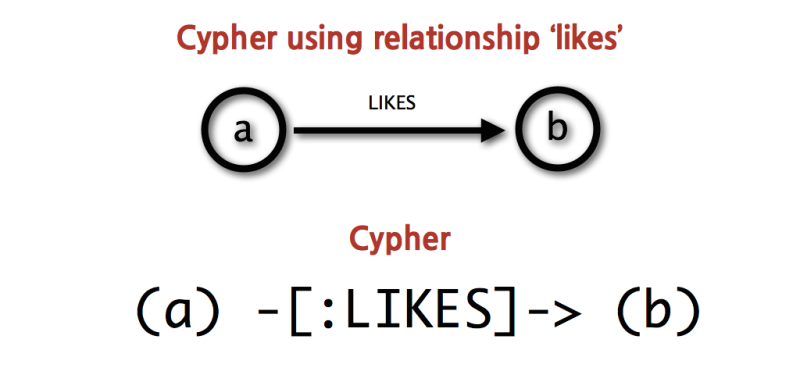
\includegraphics[width=0.6\textwidth]{../cypher_pattern_simple.png}
\caption{Cypher syntax representation of a relationship in the graph \cite{Neo4jCypher}}
\label{fig:figure29}
\end{figure}

Neo4J query language also includes a series of clauses and expressions similar to SQL, such as  $WHERE$, $ORDER BY$, $LIMIT$, $AND$, among others. The Cypher query shown in Figure \ref{fig:figure30} is an example of the general syntax of the language and it shows how it is possible to restrict the results by a certain threshold using the clause $WHERE$. The mentioned query will return a subgraph containing the nodes with labels $Label1$ and $Label2$ that have a relationship of type $TYPE$ with a property value above a certain threshold.

\begin{figure}[ht]
\centering
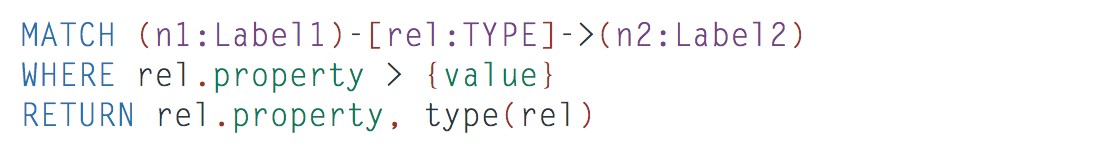
\includegraphics[width=0.8\textwidth]{../cypher_general_syntax.png}
\caption{Example of Cypher Query syntax \cite{Neo4jCypher}}
\label{fig:figure30}
\end{figure}

The data stored in a Neo4J database can be accessed using a Java API or a REST API by default. In order to facilitate the access to the data using a Python application we used an external library called Py2Neo, which wraps REST API requests to execute Cypher commands on the database. In this way, it was possible to implement the algorithm for the Graph Aggregators, where it consumes the original data, generate an aggregate graph and stores it in another instance of a Neo4J database.

Another interesting feature in Neo4J is its web-based user interface. This interface provides a direct way to submit Cypher queries to the database and a visualisation of the results. Figure \ref{fig:figure31} is a screenshot of the interface, showing the result of a simple query submitted in the text area at the top of the screen. The submitted query returns a subgraph showing the relationship between the Author Felix Naumann with all his publications present in the database. The interface shows each node as a circle and relationship as an arrow, it also shows the properties and labels of nodes and relationships when they are clicked. The experiments shown in this chapter will be displayed using the graphic interface provided by Neo4J.

\begin{figure}[ht]
\centering
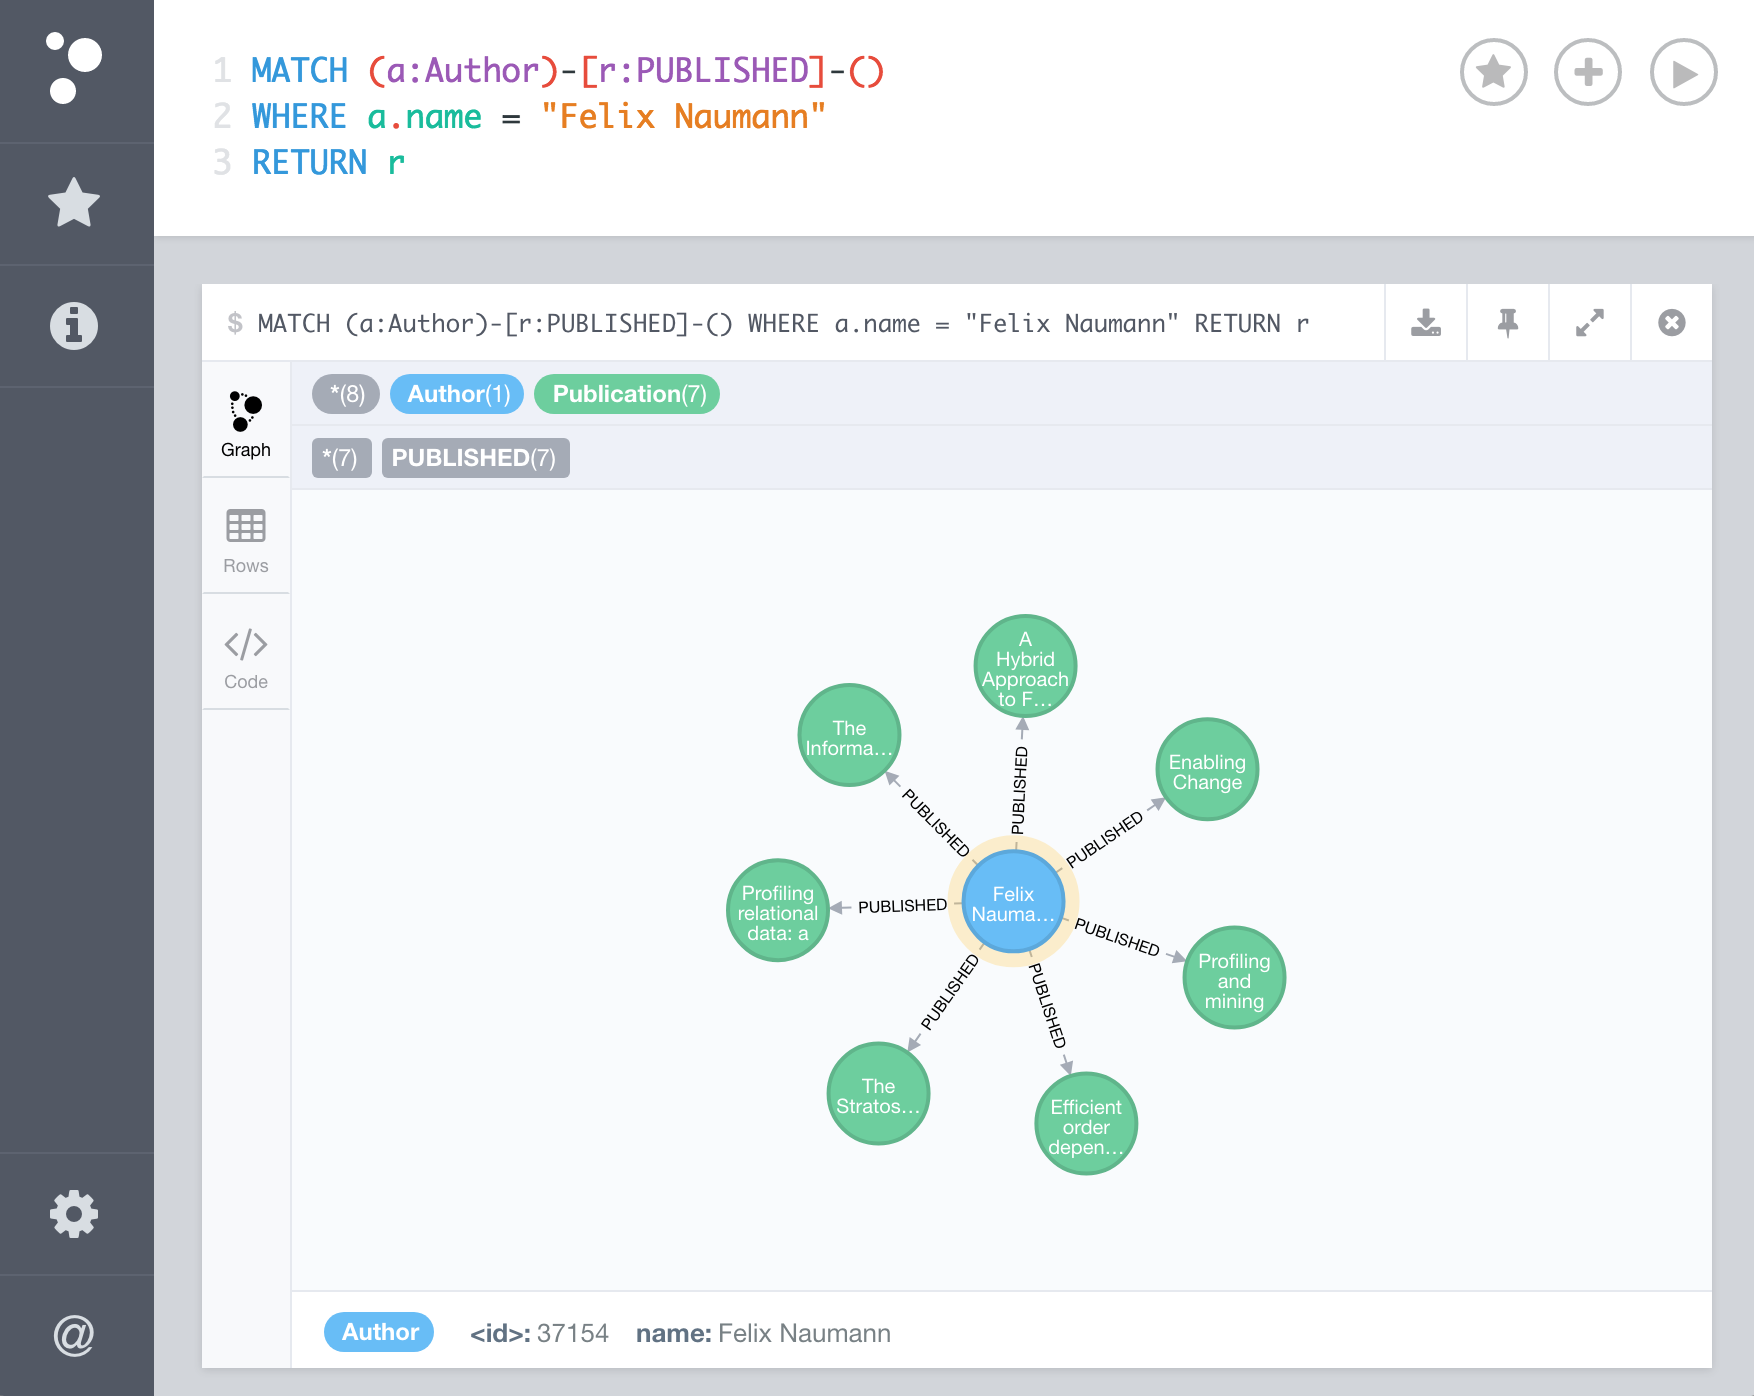
\includegraphics[width=1\textwidth]{../neo4j_user_interface.png}
\caption{Neo4J User Interface}
\label{fig:figure31}
\end{figure}


\section{Final Considerations}
In this chapter, we discussed the main concepts related to the work presented in this dissertation. Initially, the definition of Data Warehouse and Multidimensional Model were introduced, followed by a detailed view on different types and operators an OLAP system can have. Then, we covered the main components of a graph and how it can be classified according to different characteristics. Finally, we explained the definition of a Graph Database and went through a historical overview of such systems, as well as a more specific description of Neo4J database. In the next chapter, we will review the most important research published that implements an OLAP system using Graph Databases.
